\begin{figure*}[htbp]
\centering
\vspace{-0.15cm}
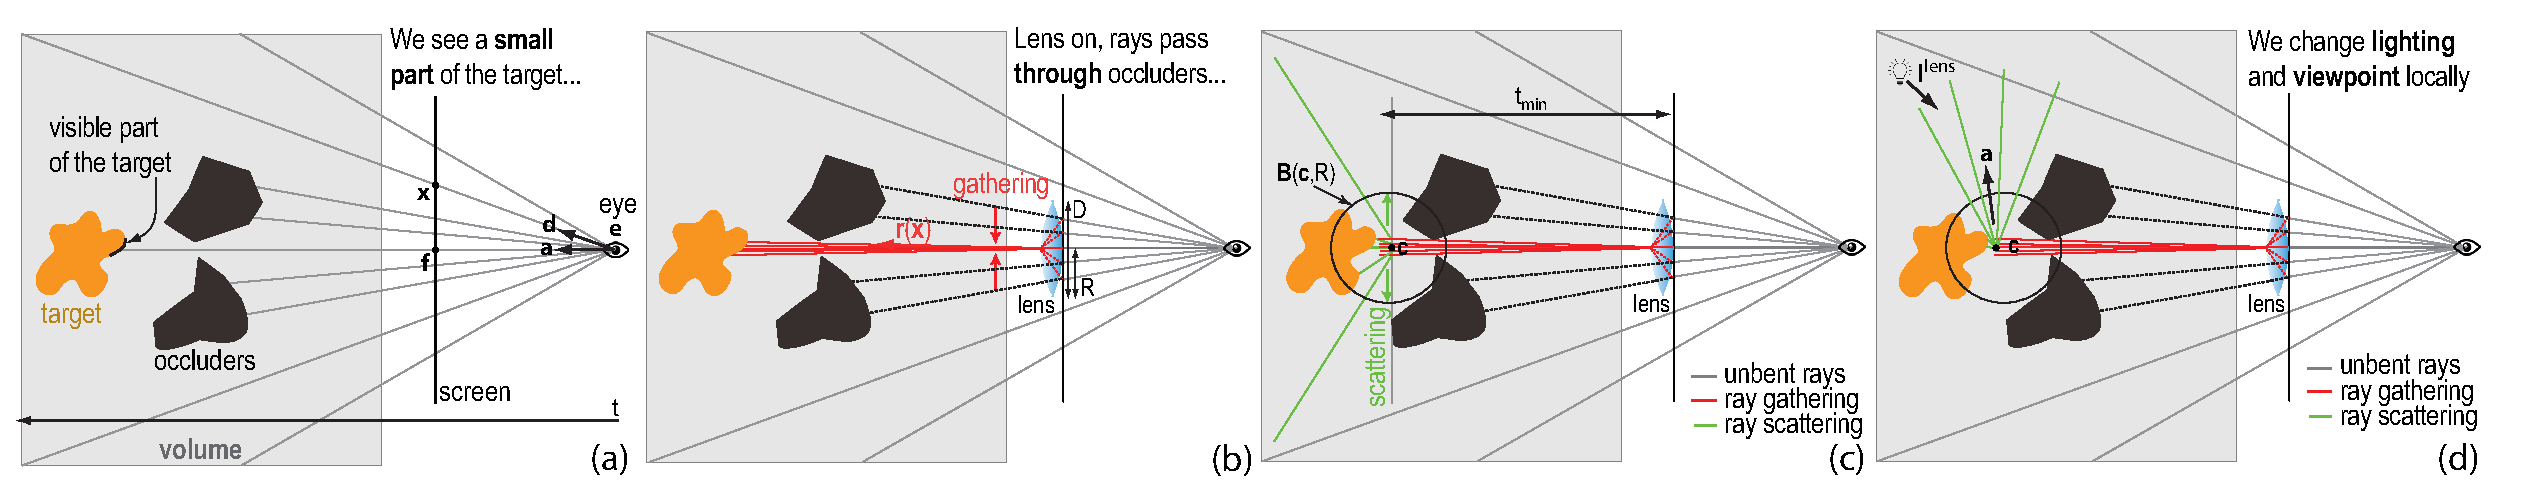
\includegraphics [width=0.94\textwidth]{images/principle.eps}
\vspace{-0.15cm}
\caption{Principle of the obstruction-free lens. An interesting target object is mostly hidden by occluders in front of it. (a) Classic raycasting result shows a small part of the target. (b) Our lens gathers the rays to avoid occluders. Once close to the target, rays follow again their initial paths. However, only a small part of the target is visible. (c) Scattering the rays makes the full target visible.}
\label{f:fisheye}
\vspace{-0.15cm}
\end{figure*}

\vspace{-0.15cm}
\section{Principle}
\label{sec:principle}
%
%
Consider the typical DVR algorithm: Given a scalar volume $V \subset \mathbf{R}^3 \rightarrow \mathbf{R}$, each pixel $\mathbf{x} \in I$ in the DVR image $I \subset \mathbf{R}^2$ thereof corresponds to the compositing of sampled data along a ray that passes through $V$ and ends at $\mathbf{x}$. In classical DVR (\autoref{f:fisheye}-a), such rays are defined by the eye position $\mathbf{e}$ and a ray direction unit vector $\mathbf{d} = (\mathbf{x} - \mathbf{e}) / \| \mathbf{x} - \mathbf{e} \|$. Consider now a focus point $\mathbf{f} \in I$ (the lens center) and a lens radius $R > 0$. We modify all rays passing through the lens (focus/0 area $D = \{\mathbf{x} \in I | \| \mathbf{x} - \mathbf{f} \| \leq R\}$ in order to de-occlude, magnify, and emphasize a target object. Our ray behavior is divided into three steps: (1) Provide a clear view of the target by moving closer to it and by pushing occluders aside. (2) Set a wide field-of-view (fisheye) to better see the target. (3) Modify the parameters of the lens, lighting, and opacity TF in real time to better explore the target. These steps are detailed next.

\subsection{Creating an unobstructed view}
\label{sec:gathering}
%
The scenario we address is as follows: Given a volume $V$, users produce a DVR thereof, using whatever suitable TFs and other parameters are applicable. When examining $V$ from various viewpoints, (at least) one viewpoint $(\mathbf{e},\mathbf{d})$ is found from which some intriguing structure is \emph{partially} visible in $I$. We call this structure the \emph{target}. Users next want to quickly and easily unravel the target. For this, we proceed as follows: We first \emph{gather} all rays passing through the lens pixels (focus area $D$) to follow the lens' axis vector $\mathbf{a} = (\mathbf{f} - \mathbf{e}) / \| \mathbf{f} - \mathbf{e} \|$. As explained above, at the location $\mathbf{f}$ of the lens center, we do see an interesting partially occluded target. Hence, by definition, the gathered rays pass \emph{through} occluders to hit this target, otherwise we would not see it. We control gathering by setting the ray direction passing through $\mathbf{x} \in D$ to
%
\begin{equation}
\mathbf{r}(\mathbf{x}) = (1-\alpha) \mathbf{a} + \alpha \mathbf{d},
\label{eqn:gathering}
\end{equation}
%
with $\alpha \in [0,1]$. When $\alpha=0$ (default), all rays follow the lens axis $\mathbf{a}$, thus, can best pass through obstacles. When $\alpha=1$, rays follow a straight path. Changing $\alpha$ with the mouse wheel smoothly navigates between the lens effect, \emph{i.e.} opening up a `hole' in the volume to see the target, and classical DVR.
%
\subsection{Setting a wide field of view}
\label{sec:scattering}
%
Once the rays pass obstacles (Sec.~\ref{sec:gathering}), we want to \emph{scatter} them so as to best sample the target. Consider that this target is at some depth $t_{target}>0$ within $V$. After the rays pass the occluders, but before they hit the target, \emph{i.e.}, travel past a distance $t_{min} < t_{target}$ through $V$, we deflect (scatter) them so as to best sample the target. For this, we set the parametric position of a ray point to
%
\begin{equation}
\mathbf{p}(\mathbf{x}, t) = \mathbf{r}(\mathbf{x})t + \beta (\mathbf{x}-\mathbf{f})(t-t_{min})
\label{eqn:scattering}
\end{equation}
%
for any pixel $\mathbf{x} \in D$ and any $t \geq t_{min}$. Here, $\beta \geq 0$, adjusted via the mouse scroll wheel while pressing the Shift key (\autoref{f:fisheye}-c), controls the ray scattering: Small values magnify a small volume area close to the ray $\mathbf{r}(\mathbf{x})$; larger values sample more of the volume behind the lens. Intuitively, this is as if we moved a magnifying lens to a depth $t_{min}$ inside $V$. Summarizing, after the user finds an interesting but partially occluded target using \emph{standard} DVR, our lens squeezes rays to pass between occluders and next fans them out to explore the target.
%
%

\vspace{-0.15cm}
\subsection{Interactive exploration of the target}
\label{sec:inter_expl}
%
To achieve a more effective exploration, we can interactively modify several parameters of the DVR and the lens, as follows.
%
\begin{figure*}[htbp]
\centering
\vspace{-0.15cm}
\includegraphics [width=0.94\textwidth]{images/params.eps}
\vspace{-0.15cm}
\caption{Changing lighting parameters in the lens. (a) Constant global specular coefficient. (b) Specular coefficient high in the lens and low outside. (c-f) Changing the in-lens light vector yields the effect of a flashlight rotating around the target. The ball icons illustrate the local light vector direction.}
\label{f:params}
\vspace{-0.15cm}
\end{figure*}
%


\vspace{0.2cm}
\noindent\textbf{Lens radius:} The radius $R$, telling how big is the `hole' to open up in the volume to see the target, is set via the mouse wheel. The parameters $\alpha$ and $\beta$ (affecting the gathering and scattering of rays respectively) are set by the mouse wheel and modifier keys. The value $t_{min}$ (depth from which scattering starts) is set using the arrow keys.

\vspace{0.2cm}
\noindent\textbf{Lens axis:} Users can rotate the lens axis $\mathbf{a}$ using a virtual trackball activated by the right mouse button. Changing $\mathbf{a}$ effectively samples the target from many viewpoints, allowing the user to look `around' it to see parts which are not visible from the current viewpoint, but \emph{without} actually changing the viewpoint. This is of high added value, since changing the viewpoint can bring us to a view where the target is fully invisible, so we do not know where precisely to activate the lens any more. Figure~\ref{f:rotation} shows three such local rotations for the baggage dataset introduced in Fig.~\ref{f:baggage_lens}. From these, we see that the star-shaped target is relatively thick.

\vspace{0.2cm}
\noindent\textbf{Lighting:} We modify the volumetric Phong lighting parameters to better explore the target, as follows. Let $\mathbf{c} = \mathbf{e} + t_{min}\mathbf{a}$ be a point at depth $t_{min}$ along the lens axis, and let $B(\mathbf{c},R)$ be a sphere of radius $R$ around this point (\autoref{f:fisheye}b). We call voxels in this sphere `in focus', and all other voxels in $V$ `out of focus'. Let $\phi$ be the specular term coefficient, set to a high value (default: one).
First, for all voxels $\mathbf{x} \in B(\mathbf{c},R)$, we use a specular coefficient $\phi(\mathbf{x}) = \phi (1-d)$, where $d=\|\mathbf{x}-\mathbf{c}\|/R$. For all voxels outside $B(\mathbf{c},R)$, we use $\phi(\mathbf{x}) = 0$. Hence, voxels close to the focus point $\mathbf{c}$ appear highly specular; further away from $\mathbf{c}$, voxels get less specular, and voxels out of focus are purely diffuse. Secondly, we allow the user to locally rotate the light vector using the same trackball mechanism as for the lens axis rotation. Let $\mathbf{l}^{lens}$ be this vector, and let $\mathbf{l}^{global}$ be the global light vector used by standard DVR. For all voxels in focus, we use a light vector $\mathbf{l}(\mathbf{x}) = (1 - d)\mathbf{l}^{lens} + d\mathbf{l}^{global}$. As the user rotates $\mathbf{l}^{lens}$, the light direction will visibly change in the middle of the lens, stay constant outside it, and smoothly change in between.

The above two mechanisms combined yield the effect of a moving flashlight turning around a shiny target embedded in a constantly-lit diffuse scene. Figure~\ref{f:params} shows these mechanisms for a chest CT dataset containing a deeply buried tumor (the dataset and use-case are described in detail in Sec.~\ref{sec:chest}). We see how turning the light highlights small-scale details on the target surface (tumor) without changing the viewpoint or lens location. Moreover, the high specularity in the lens attracts the user's attention to this area; the diffuse lighting outside the lens put less emphasis on the context area. 

\vspace{0.2cm}
\noindent\textbf{Opacity:} We modify the opacity transfer function along a similar idea as for lighting (Fig.~\ref{fig:tf}). Let $TF_{o}^{global} : \mathbf{R} \rightarrow [0,1]$ be the user-chosen opacity function used globally for the volume. Let $\Gamma$ be a Gaussian pulse of unit height centered at the average density value $\bar{\rho}$ in $B(\mathbf{c},R)$ and with standard deviation $\sigma$. We estimate $\bar{\rho}$ and $\sigma$ by considering the density $\rho$ at 150 points randomly sampled inside $B(\mathbf{c},R)$. Higher values for the sample count yield visually very similar results, while require (slightly) more computation costs. Then, for voxels in $B(\mathbf{c},R)$, we use an effective opacity transfer function $TF_o = TF_{o}^{global} + (1-d) \Gamma$. For voxels outside $B$, we use $TF_{o}^{global}$ (standard DVR). The effect is that voxels in $B$ become more opaque, thus more visible. Voxels with the same densities but outside $B$ use the default transfer function, which can make them transparent. This makes voxels with similar densities either opaque (if close to the target, thus of interest) or transparent (if \emph{e.g.} in front of the target, thus occluding). Figure~\ref{f:params} has been generated this way. 


%ALEX: This phrase was indeed confusing, I don't know what we wanted to say with it: 
%We see here how the tumor in the lens has the same opacity as the muscle tissue outside the lens, even though the two have nearly identical densities.

\begin{figure}[htbp!]
\centering
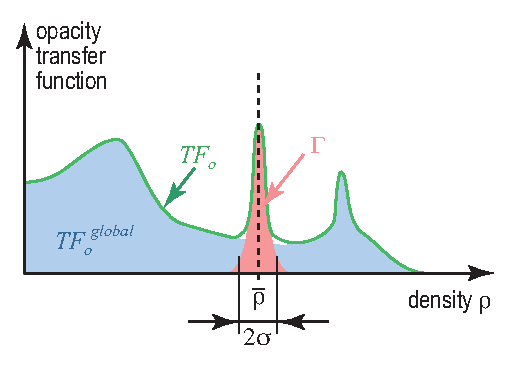
\includegraphics[width=0.29\textwidth]{images/tf.eps}
\vspace{-0.15cm}
\caption{Construction of local transfer function $TF_{o}$. See Sec.~\ref{sec:inter_expl}.}
\vspace{-0.15cm}
\label{fig:tf}
\end{figure}


\subsection{Smooth transitions}
\label{continuity}
%
If we bend rays passing through the lens pixels $D$ (Eqns.~\ref{eqn:gathering} and~\ref{eqn:scattering}) and trace rays starting at pixels in $I \setminus D$ as straight lines, discontinuities appear at the lens borders. We solve this as follows. Let $\mathbf{p}(\mathbf{x},t)$ be the voxels along a lens ray starting at screen pixel $\mathbf{x}$, as computed by Eqn.~\ref{eqn:scattering}. Let $\mathbf{p}^{line}(\mathbf{x},t)$ be the voxels along a straight-line ray starting at $\mathbf{x}$, \emph{i.e.}, computed using $\alpha=1$ and $\beta=0$ in Eqns.~\ref{eqn:gathering} and~\ref{eqn:scattering} respectively. For every value $t$ along every such ray, we compute the interpolated ray $\bar{\mathbf{p}}(\mathbf{x},t) = (1-f(d))\mathbf{p}(\mathbf{x},t) + f(d)\mathbf{p}^{line}(\mathbf{x},t)$, where $d$ is the distance of $\mathbf{x}$ to the lens axis (normalized to unit by dividing it by $R$) and $f : [0,1] \rightarrow [0,1]$ is an interpolation function. Next, we use the rays $\bar{\mathbf{p}}(\mathbf{x},t)$ to compute the DVR by standard composition. This way, rays effectively vary smoothly from their bent versions (close to the lens axis) to straight lines (outside the lens). Setting $f(d) = d^2$ keeps the interpolation transitions close to the lens border, so most of the lens is dedicated to show the desired fisheye effect.

\begin{figure}[htbp!]
\centering
\includegraphics [width=0.42\textwidth]{images/rotation.eps}
\vspace{-0.15cm}
\caption{Performing local rotations in the lens allows better seeing the shape and thickness of the partially occluded target object (ninja star).}
\label{f:rotation}
\vspace{-0.15cm}
\end{figure}

Separately, we use a slow-in/slow-out animation\,\cite{Dragicevic:2011:TDA:1978942.1979233} to introduce the lens effect. When activating the lens, we vary $\alpha$ and $\beta$ from their defaults ($\alpha=1$, $\beta=0$, \emph{i.e.} straight-line classical DVR) to their actual user-set values, compute the volume rendering on-the-fly, and display the resulting images. The effect resembles gradually opening a hole in the volume -- see the associated video. The speed increase at the start of the animation helps one to quickly see what is revealed in the lens; the decreasing speed at the end helps seeing where the pushed-away occluders actually go. This also gives some semantic to the moving shapes, allowing one to interpret the motion as a magnification of a target, and to keep the focus on visual entities during this transition. When deactivating the lens, we play back the animation in the opposite sense, which suggests closing the opened hole in the volume.

\section{Implementation}
\label{sec:implem}
%
We implemented our occlusion-free lens by modifying a standard DVR ray caster, publicly available in NVIDIA CUDA's SDK\,\cite{cudasdk}. We modified this ray caster to incorporate the new ray definition (Eqns.~\ref{eqn:gathering} and \ref{eqn:scattering}), the lens effect, and the local per-voxel Phong lighting parameters, all controlled via keyboard and mouse. On a PC with 16 GB RAM and a GeForce GTX TITAN X card, we achieve 15 frames per second for volumes up to $512^3$ voxels at a $1900 \times 1200$ pixels screen resolution. Currently, we use a compositing ray function. Any other functions can be directly used with no restrictions. All in all, adding our lens to an existing ray caster should pose no significant implementation problems.

\begin{comment}
%ALEX: Commented out the algo pseudocode. There are so far several problems with it, needs to be rewritten, anyways using the current notations. We can see if we have space/time to do it when all else is ready.

Algorithm \ref{alg:propagation} shows a pseudo code of the behavior of our deforming lens

\begin{algorithm}
\SetKwInOut{Input}{Input}
\SetKwInOut{Output}{output}
\SetKwInOut{Parameter}{Parameter}

 \Input{
 $\vec{e}$: the eye position,
 
 $\vec{d}\left(x,y\right)$: the ray direction according to the screen space coordinates of the resulting pixel ($x$ and $y$),
 
 $step$: the sampling distance along the ray.
 
 }
 \KwResult{the pixel color.}
 
 \Parameter{
 $a$: the attraction factor,
 
 $\alpha$: the angle of view.
 }
\BlankLine
 
  $k  \leftarrow $ the normalized distance to the axis of the lens
 $\vec{p}_{near}  \leftarrow \vec{e} + t_{near} \times \vec{d}\left(x,y\right)$ //The initial position  \; 
 $\vec{p}^{0} \leftarrow \vec{p}_{near} $ \; 
 \While{ $ t \le t_{far}$ And $Opacity \le Opacity Threshold  $ }{
 	\If{the current ray is inside the lens}{
    	\If{ $t < t_{target}$ }{
        	$\vec{p}^{1} \leftarrow \vec{p}_{near}\left(x,y\right) + t \times \vec{d}_{target} + a \times \vec{f}_{attraction}$  \;
            \lElse{
        	$\vec{p}^{1} \leftarrow \vec{p}_{target} + \left( t-t_{target} \right) \times \vec{d}_{fishEye}\left( \alpha \right)$
        	}	
        }
               
    $\vec{p} \leftarrow \vec{p}^{0} + f\left(k\right) \times \left( \vec{p}^{1} - \vec{p}^{0} \right) $	\;
     \lElse{
     	 $\vec{p} \leftarrow \vec{p}^{0}$
     }
    }
\emph{Sampling at the position $\vec{p} $ }\;
    
    \emph{Shading the sampled value }\;
    
    \emph{ Compositing the shaded sampling point with the previous values} \;
 
    $t \leftarrow t + step$ \;
    $p^{0} \leftarrow p^{0} + step \times \vec{d}\left(x,y\right)$ \;

}
$color_{final} \leftarrow$ composited colors \;
return $color$
 

\label{alg:propagation}
 \caption{Pseudo code of our lens deformation algorithm}
\end{algorithm}

\end{comment}


